\subsection{Geographic Spread}
\label{sect:geospread}

Here we examine each cluster's geographic spread --- the closeness, in terms of
geographic distance, of members of the same cluster. As clients sharing the same
cluster are predominantly exposed to the same network resources, the geographic
spread of a cluster's clients must related to the network performance (latency)
they experience. Specifically, if a pair of clients directed
to the same network resource are physically ``far'' apart from each other, it is
likewise impossible for \emph{both} clients to simultaneously be near said
resource. In such an arrangement, the resource is either near one client and far from the other, or the
resource is equidistant from both clients. In the latter case, if the clients
are sufficiently far from each other, the resource must also far from both clients.

To calculate these geographic distances, we use coordinates for RIPE Atlas
probes --- our client machines in the context of this experiment --- obtained
from RIPE Atlas's API. RIPE acquires probe location information via manual input
from volunteers who themselves maintain Atlas probes, and, where necessary, by
autmated input from MaxMind CITE. Figure \ref{geomeans} shows the CDF of the
mean geographic distance (in kilometers) between members of a cluster, for each
cluster. Members of a cluster with a larger mean geographic distance are farther
apart form each other, on average, than are the members of a cluster with a
lower mean geographic distance. In the median case, we see an average client
distance of 509 km. We observe that for 20\% of clusters, members are over 1000
km on average. For perspective, we remind the reader that the circumference of
the world is approximately 40,075 km. 

\begin{figure}
    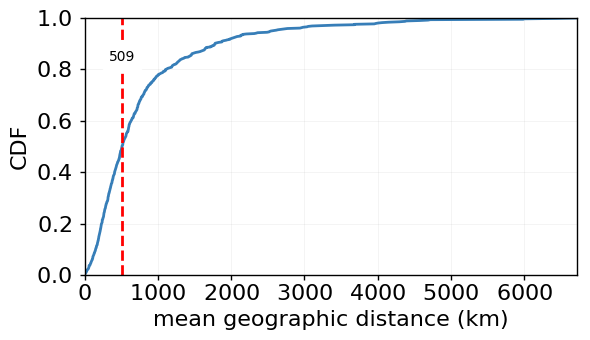
\epsfig{file=figs/geo_means.png, width=1\linewidth}
    \caption{CDF of mean geographic distance between
    cluster members. The dashed vertical line marks the median.}
    \label{geomeans}
\end{figure}

Since CNRE potentially spans many, physically distinct resources, it serves as
an \emph{aggregate} measurement, and we do not attempt to pinpoint the location
of any individual resource. Instead, we identify the effective ``center'' of
each cluster and measure the effect of a member's distance from the center.
Following the intuition of CDN deployment laid out in other work (CITE), we
hypothesize that the geographic center of a cluster will sit physically close
the location of the most of that cluster's network resources. By this logic,
clients closer to their cluster's center should experience better network
performance (\emph{i.e.}, lower latency) than those farther away. To test this,
we compared each client's mean latency (taken across all 299 ping responsive domains
in our set) to that client's distance from its respective cluster's center. For
simplicity, we use a cluster's geometric median as an estimate of its center.
The results of this comparison are shown in Figure \ref{geoperf} as a scatter
plot of mean latency versus distance from cluster center. Each point corresponds
to a single client's latency and distance from its respective cluster's center.
The figure also includes a best fit line, denoting the overall trend of the
points. 

Note the positive slope of points in Figure \ref{geoperf}, indicative of a
directly proportional relationship between latency and distance from the
cluster's effective center. As a client's distance from its cluster's center
increases, so does its latency. Performance for clients relatively near their
respective centers --- closer than 1000 km --- is seemingly noisy and no trend
is clearly observable.  However, as the geographic distance increases beyond
1000 km, the directly proportional relationship between performance and center
distance becomes more apparent. 

We also point out that the slope of Figure \ref{geoperf}'s the
best line quantifies this relationship approximately
8.2\texttimes10\textsuperscript{7}m/s, which implies a general data speed of
$\frac{1}{4}$ of the speed of light. This finding similar that of CITE. In additon, the
fastest network communication mediums in use at the time of this writing move
data at approximately $\frac{2}{3}$ of the speed of light CITE. Accounting for
traffic, routing complexity, and the pressence of lower speed mediums may
account for our lower finding.

\begin{figure}
    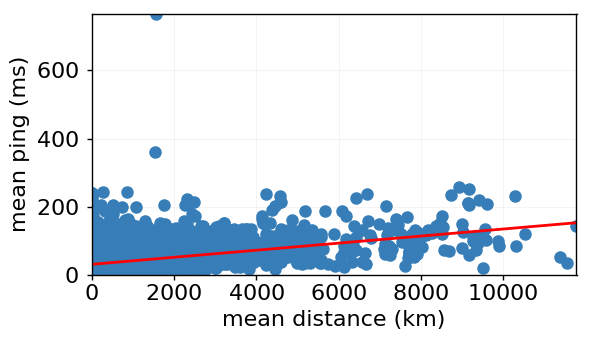
\epsfig{file=figs/geo_vs_perf.png, width=1\linewidth}
    \caption{Scatter plot where, for each client, we compares the client's mean latency
    (across all responding sites) to that client's distance from its cluster's
    center. The line denotes a first order best fit curve for the scatter plot's points.}
    \label{geoperf}
\end{figure}
